\documentclass[aspectratio=169]{beamer}

\usepackage[titlebg=thwsorange,
authorcolor=black,
titlecolor=white,
bc=thwsorange,
nospeakerspace,
slidenumber,
bs=$\bullet$]{thwsbeamertheme}

\usetikzlibrary{arrows.meta,positioning,calc}
\usepackage{ragged2e}
\usepackage{pgfpages}
\setbeameroption{show notes on second screen=right}

\title{Interaktive Lernplattform\\für\\Grundlagen Informatik}
\author{M. Nöth, R. Schröder, E. Ebert, D. T. Pham, K. Popov}
\modulename{Projektarbeit}
\date{Projektpräsentation}

\tikzset{
  diagramnode/.style={
    rounded corners=2mm,
    fill=thwsgrey,
    text=black,
    align=center,
    inner xsep=5mm,
    inner ysep=4mm,
    minimum height=1.15cm,
    font=\large
  },
  diagramarrow/.style={
    -{Latex[length=3.2mm,width=2.1mm]},
    draw=thwsorange,
    line width=1.6pt
  },
  diagramdouble/.style={
    {Latex[length=3.0mm,width=2.0mm]}-{Latex[length=3.0mm,width=2.0mm]},
    draw=thwsorange,
    line width=1.6pt
  }
}

\begin{document}

\begin{frame}
  \titlepage
\end{frame}

\addsectionframe{1. Kontext und Zielbild}

\begin{contentsframe}{Problemstellung}
\vfill
\centering
\resizebox{0.84\textwidth}{!}{%
\begin{tikzpicture}[node distance=7mm and 7mm]
  \node[diagramnode, minimum width=3.8cm] (abstract)
    {Abstrakte, dynamische\\Fachmodelle};

  \node[diagramnode, below left=of abstract, minimum width=3.5cm] (static)
    {Statische\\Lehrmaterialien};

  \node[diagramnode, below right=of abstract, minimum width=3.5cm] (practice)
    {Wenig interaktives\\Experimentieren};

  \node[diagramnode, below=9mm of abstract, yshift=-12mm, minimum width=4.3cm] (steps)
    {Zwischenschritte schwer\\nachvollziehbar};

  \node[diagramnode, below=6mm of steps, minimum width=4.6cm] (need)
    {Lernbedarf: sichtbar,\\veränderbar, direktes Feedback};
  \draw[diagramarrow] (abstract) -- (static);
  \draw[diagramarrow] (abstract) -- (practice);
  \draw[diagramarrow] (static) -- (steps);
  \draw[diagramarrow] (practice) -- (steps);
  \draw[diagramarrow] (steps) -- (need);
\end{tikzpicture}%
}
\vfill

\note{
  \textbf{Person: }

  \textbf{Zeit: 3 bis 5 min}

  \begin{itemize}
    \item test
    \item test
    \item test
  \end{itemize}
}
\end{contentsframe}


\begin{itemframe}{Ziele der Plattform}
  \item Browserbasierte Lern- und Übungsplattform
      \vspace{1em}
  \item Überblick, Beispiele, Übungen und freie Simulation
      \vspace{1em}
  \item Einheitliche Bedienung, Mehrsprachig und helle / dunkel Darstellung
  \note{
    \textbf{Person: }

    \textbf{Zeit: 1 bis 2 min}

    \begin{itemize}
      \item test
      \item test
      \item test
    \end{itemize}
  }
\end{itemframe}

\addsectionframe{2. Anforderungen und Projektablauf}

\begin{itemframe}{Anforderungen}
  \item Didaktik: interaktive Simulatoren und direktes Feedback
      \vspace{1em}
  \item Bedienung: intuitiv, einheitlich und konsistent
      \vspace{1em}
  \item Technik: modularer Aufbau / Erweiterbarkeit, browserbasiert
      \vspace{1em}
  \item Qualität: Wartbarkeit, fachliche Korrektheit und Reproduzierbarkeit, sinnvoller Umgang mit KI
  \note{
    \textbf{Person: }

    \textbf{Zeit: 2 min}

    \begin{itemize}
      \item test
      \item test
      \item test
    \end{itemize}
  }
\end{itemframe}

\begin{itemframe}{Zusammenarbeit und Feedback-Zyklen}
  \item Agil orientierte, iterative Arbeitsweise
        \vspace{1em}
  \item Wöchentliches Teammeeting
        \vspace{1em}
  \item Git, GitLab, Work Items und Milestones
        \vspace{1em}
  \item Regelmäßiges Auftraggeber-Feedback
    \note{
      \textbf{Person: }

      \textbf{Zeit: 1 bis 2 min}

      \begin{itemize}
        \item test
        \item test
        \item test
      \end{itemize}
    }
\end{itemframe}

\addsectionframe{3. Lösungsansatz: Architektur und Design}

\begin{itemframe}{Technische Basis}
  \item React 19 + TypeScript + React Router
          \vspace{1em}
  \item Vite + Tailwind CSS 4 + shadcn/ui
          \vspace{1em}
  \item Zustand + i18next
          \vspace{1em}
  \item Monaco + OpenJDK javac + TeaVM
    \note{
      \textbf{Person: }

      \textbf{Zeit: 1 min}

      \begin{itemize}
        \item test
        \item test
        \item test
      \end{itemize}
    }
\end{itemframe}

\begin{itemframe}{Modulare Plattformarchitektur}
  \item Fachlich getrennte Topics
          \vspace{1em}
  \item Gemeinsame Shared Components
          \vspace{1em}
  \item \texttt{moduleCatalog.tsx} als zentrale Modulverwaltung
    \note{
      \textbf{Person: }

      \textbf{Zeit: 1 min}

      \begin{itemize}
        \item test
        \item test
        \item test
      \end{itemize}
    }
\end{itemframe}

\begin{itemframe}{Unified UI: wiederkehrendes Design}
  \item Header, Sidebar, Footer und Content
          \vspace{1em}
  \item Pro Topic: Überblick, Übungen, Beispiele und Simulation
          \vspace{1em}
  \item Gemeinsame Komponenten
          \vspace{1em}
  \item Fachspezifische Visualisierung in jedem Topic
    \note{
      \textbf{Person: }

      \textbf{Zeit: 1 min}

      \begin{itemize}
        \item test
        \item test
        \item test
      \end{itemize}
    }
\end{itemframe}

\begin{contentsframe}{Simulator-Architektur}
\centering
\vspace{1mm}
\resizebox{0.88\textwidth}{!}{%
\begin{tikzpicture}[node distance=9mm and 7mm]
  \node[diagramnode, minimum width=3.3cm, font=\normalsize] (data) {Konfiguration +\\Laufzeitzustand};
  \node[diagramnode, right=of data, minimum width=4.0cm, font=\normalsize] (iface) {\texttt{ISimulator<TConfig,TState>}\\gemeinsames Interface};
  \node[diagramnode, right=of iface, minimum width=3.7cm, font=\normalsize] (hook) {\texttt{useSimulationEngine}\\Steuerung + Synchronisation};
  \node[diagramnode, below=of hook, minimum width=3.7cm, font=\normalsize] (ui) {React-UI\\Play / Pause / Step / Reset};
  \node[diagramnode, below=of iface, minimum width=4.0cm, font=\normalsize] (impl) {Konkrete Simulatorlogik};

  \draw[diagramarrow] (data) -- (iface);
  \draw[diagramarrow] (iface) -- (hook);
  \draw[diagramarrow] (iface) -- (impl);
  \draw[diagramdouble] (impl) -- (hook);
  \draw[diagramdouble] (hook) -- (ui);
\end{tikzpicture}%
}
  \note{
    \textbf{Person: Richard}

    \textbf{Zeit: 2 bis 3 min}

    \begin{itemize}
      \item test
      \item test
      \item test
    \end{itemize}
  }
\end{contentsframe}

\begin{itemframe}{Import, Export und lokale Persistenz}
  \item Gemeinsamer Transfer-Codec
          \vspace{1em}
  \item Kompakte Base64URL-Transferstrings
          \vspace{1em}
  \item Local Storage
    \note{
      \textbf{Person: Markus}

      \textbf{Zeit: 1 bis 2 min}

      \begin{itemize}
        \item test
        \item test
        \item test
      \end{itemize}
    }
\end{itemframe}

\addsectionframe{4. KI-Einsatz im Projekt}

\begin{itemframe}{KI-Werkzeuge im Projekt}
  \item Stitch, ChatGPT, Gemini, Claude, Codex, Antigravity, verschiedene OpenCode und lokale Modelle
            \vspace{1em}
  \item MCP, LSP, Graphify und Agent Skills
    \note{
      \textbf{Person: }

      \textbf{Zeit: 1 min}

      \begin{itemize}
        \item test
        \item test
        \item test
      \end{itemize}
    }
\end{itemframe}

\begin{contentsframe}{Arbeitsweise: KI als Co-Developer}
\centering
\vspace{2mm}
\begin{tikzpicture}[node distance=8mm and 11mm]
  \node[diagramnode, minimum width=3.7cm] (context) {Mensch: Aufgabe +\\Architekturkontext};
  \node[diagramnode, right=of context, minimum width=3.5cm] (plan) {KI: Analyse\\und Plan};
  \node[diagramnode, right=of plan, minimum width=3.6cm] (change) {KI: Änderungs-\\vorschlag};
  \node[diagramnode, below=of change, minimum width=3.6cm] (review) {Mensch: Diff +\\Fachreview};
  \node[diagramnode, left=of review, minimum width=3.5cm] (tests) {Mensch / KI: Tests +\\Browserprüfung};

  \draw[diagramarrow] (context) -- (plan);
  \draw[diagramarrow] (plan) -- (change);
  \draw[diagramarrow] (change) -- (review);
  \draw[diagramarrow] (review) -- (tests);
  \draw[diagramarrow] (tests.north) -- (plan.south);
\end{tikzpicture}
  \note{
    \textbf{Person: }

    \textbf{Zeit: 2 min}

    \begin{itemize}
      \item test
      \item test
      \item test
    \end{itemize}
  }
\end{contentsframe}

\begin{itemframe}{Grenzen und Erkenntnisse beim KI-Einsatz}
  \item Kontextverlust bei großen Aufgaben $\rightarrow$ \texttt{handover.md}
              \vspace{1em}
  \item Duplikate und toter Code $\rightarrow$ Code Review mit KI
              \vspace{1em}
  \item Nutzen durch kleine, testbare Schritte
    \note{
      \textbf{Person: }

      \textbf{Zeit: 2 min}

      \begin{itemize}
        \item test
        \item test
        \item test
      \end{itemize}
    }
\end{itemframe}

\addsectionframe{5. Qualität und Deployment-Strategie}

\begin{itemframe}{Qualitätssicherung}
  \item ESLint + Prettier + fallow
                \vspace{1em}
  \item Vitest
                \vspace{1em}
  \item Vite Build + Playwright + MCP
                \vspace{1em}
  \item Lighthouse + manuelles Review
    \note{
      \textbf{Person: }

      \textbf{Zeit: 1 min}

      \begin{itemize}
        \item test
        \item test
        \item test
      \end{itemize}
    }
\end{itemframe}

\begin{itemframe}{Deployment}
  \item Statischer Vite-Build als ZIP ausgeliefert
  \vspace{1em}
  \item Browserbetrieb durch lokalen Server
  \vspace{1em}
  \item Online hosting durch Auftraggeber abgelehnt
    \note{
      \textbf{Person: }

      \textbf{Zeit: 1 min}

      \begin{itemize}
        \item test
        \item test
        \item test
      \end{itemize}
    }
\end{itemframe}

\addsectionframe{Fachmodul: Turingmaschine}

% ---------------------------------------------------------------------------
\begin{itemframe}{Turingmaschine -- Überblick}
  \item Meine Erklärung
\end{itemframe}

% ---------------------------------------------------------------------------
% Fachmodul Endliche Automaten (Kristian Popov)
% ---------------------------------------------------------------------------

\addsectionframe{Fachmodul: Endliche Automaten}

% ---------------------------------------------------------------------------
\begin{itemframe}{Endliche Automaten -- Überblick}
  \item \textbf{DFA} und \textbf{NFA} selbst definieren
  \item \textbf{Rechtslineare Grammatik} $\rightarrow$ \textbf{Automat}
  \item Zwei Sichten: \textbf{Übergangstabelle} und \textbf{Zustandsdiagramm}
  \item \textbf{Stapeltest} für mehrere Wörter gleichzeitig
  \item \textbf{Schritt-Historie}: vorwärts, rückwärts, zu einem früheren Schritt
  \item \textbf{Übungen} mit Rückmeldung: korrekt, falsch, Gegenbeispiel

  \note{
          \textbf{Person: Kristian}

          \textbf{Zeit: 1,5 min}

          \begin{itemize}
            \item Automat selbst definieren: Typ, Alphabet, Zustände, Startzustand, Endzustände,
            Übergänge und testen ihn anschließend mit einem Testwort.
            \item \textbf{Grammatik} $\rightarrow$ \textbf{Automat}: Man kann eine RL Grammatik eingeben und\ldots.
            Jedes Nichtterminal wird Zustand, jede Produktion wird Übergang
            \item \textbf{Zwei Sichten}: Tabelle und Diagramm zeigen denselben Schritt, immer synchron
            \item \textbf{Stapeltest}: Prüft mehrere Wörter auf einmal.
            \item \textbf{Schritt-Historie}: Vorwärts rückwärts oder zu einem bestimmten Schritt springen.
            \item \textbf{Übungen}: Übungen werden automatisch korrigiert.
            Dabei prüft das System das Verhalten des Automaten und bei Fehlern zeigt direkt das erste falsche Wort als Gegenbeispiel an.
          \end{itemize}
  }
\end{itemframe}

% ---------------------------------------------------------------------------
\begin{fullframe}{Simulationsschritt}
  \begin{center}
  \resizebox{0.98\textwidth}{!}{%
    \begin{tikzpicture}[
        >=Stealth,
        stepbox/.style={draw=thwsblue, very thick, rounded corners=3pt, fill=thwsblue!5,
                        minimum width=32mm, minimum height=10mm, align=center, font=\small},
        exitbox/.style={draw=thwsblue!55, thick, rounded corners=3pt, fill=white,
                        minimum width=36mm, minimum height=9mm, align=center,
                        font=\scriptsize, text=thwsblue},
        histbox/.style={draw=thwsorange, very thick, rounded corners=4pt, fill=thwsorange!8,
                        minimum width=62mm, minimum height=12mm, align=center, font=\small},
        viewbox/.style={draw=thwspetrol, very thick, rounded corners=3pt, fill=thwspetrol!8,
                        minimum width=40mm, minimum height=10mm, align=center, font=\small}
      ]

      % --- (1) der Kern: immer dieselbe Schleife
      \node[stepbox] (in)   at (-4.9, 2.4) {aktive Zustände\\+ nächstes Symbol};
      \node[stepbox] (look) at ( 0.0, 2.4) {Übergänge\\nachschlagen};
      \node[stepbox] (out)  at ( 4.9, 2.4) {neue aktive\\Zustände};

      \draw[->, very thick, thwsblue] (in)   -- (look);
      \draw[->, very thick, thwsblue] (look) -- (out);

      \draw[->, thick, thwsblue!70] (out.north) -- ++(0, 0.6)
        -- node[font=\scriptsize, above, text=thwsblue] {nächstes Zeichen} ($(in.north)+(0, 0.6)$)
        -- (in.north);

      % --- (2) wie ein Lauf endet: eigene Kaesten mit Pfeil statt freier Text
      \node[exitbox] (dead) at (0.0, 0.85) {kein Übergang:\\Wort abgelehnt};
      \node[exitbox] (fin)  at (4.9, 0.85) {Wort zu Ende:\\Endzustand aktiv?};

      \draw[->, thick, thwsblue!55] (look.south) -- (dead.north);
      \draw[->, thick, thwsblue!55] (out.south)  -- (fin.north);

      % --- (3) der Schritt wird angehaengt, nicht ueberschrieben
      \node[histbox] (hist) at (0, -1.05)
        {Schritt wird an die \textbf{Historie} angehängt\\[0.4ex]
         {\scriptsize der vorherige Schritt bleibt unverändert}};

      \draw[->, very thick, thwsorange] (out.east) -- ++(1.25, 0) |- (hist.east);

      % --- (4) eine Quelle, zwei Sichten
      \node[viewbox] (tab)  at (-3.0, -2.95) {Übergangstabelle\\{\scriptsize markierte Zelle}};
      \node[viewbox] (diag) at ( 3.0, -2.95) {Zustandsdiagramm\\{\scriptsize markierte Kante}};

      \draw[->, very thick, thwspetrol] (hist.south) -- (tab.north);
      \draw[->, very thick, thwspetrol] (hist.south) -- (diag.north);

      \node[font=\scriptsize, text=thwspetrol, fill=white, inner sep=0.6mm] at (0, -2.1)
        {beide lesen denselben Schritt};
    \end{tikzpicture}%
  }
  \end{center}

  \note{
        \textbf{Person: Kristian}

        \textbf{Zeit: 1 min}

        \begin{itemize}
          \item \textbf{Aktive Zustände} + \textbf{nächstes Symbol}
          $\rightarrow$ passende Übergänge suchen.
          \item Daraus entstehen die neuen aktiven Zustände
          \item Nächstes Zeichen beginnt der Ablauf wieder von vorne.
          \item Zwei Ausgänge: kein Übergang $\rightarrow$ abgelehnt.
                Wortende $\rightarrow$ Endzustand entscheidet.
          \item \textbf{Historie}: jeder Schritt gespeichert
                $\rightarrow$ vor- und zurückspringen.
          \item Tabelle und Diagramm zeigen denselben Schritt, immer synchron.
        \end{itemize}
  }
\end{fullframe}

% ---------------------------------------------------------------------------
% Fachmodul Reguläre Sprachen (Kristian Popov)
% ---------------------------------------------------------------------------

\addsectionframe{Fachmodul: Reguläre Sprachen}

% ---------------------------------------------------------------------------
\begin{itemframe}{Reguläre Sprachen -- Überblick}
  \item \textbf{Rechtslineare Grammatik} selbst definieren.
  \item Drei Modi: \textbf{Aufzählung}, \textbf{Erzeugung}, \textbf{Worterkennung}
  \item Sprache als \textbf{Wortliste} oder in \textbf{Mengenschreibweise}: $\{a^n b \mid n \geq 1\}$
  \item Erzeugte Grammatik \textbf{ausführlich} oder \textbf{vereinfacht}
  \item \textbf{Worterkennung} für mehrere Wörter -- mit Begründung statt nur ja/nein
  \item \textbf{Übungen} mit Rückmeldung: fehlende und falsche Wörter
          \note{
            \textbf{Person: }

            \textbf{Zeit:  min}

            \begin{itemize}
              \item Einstiegsfolie des zweiten Themas, parallel zum Überblick bei den Automaten.
              \item Nur benennen, was die Studierenden tun können -- die Begründungen kommen auf den
              \item folgenden Folien.
              \item Die drei Modi heißen in der Oberfläche "Grammatik -> Sprache", "Sprache -> Grammatik"
              \item und "Wort erkennen"; die nächste Folie vertieft sie.
              \item Ausführlich/Vereinfacht: ein Nichtterminal pro Präfix gegenüber zusammengefassten
              \item Nichtterminalen mit denselben Fortsetzungen -- rechtslinear bleiben beide.
              \item Überleitung: "Diese drei Arbeitsweisen im Zusammenhang."
            \end{itemize}
          }
\end{itemframe}
\note{%

}

% ---------------------------------------------------------------------------
\begin{fullframe}{Reguläre Sprachen -- drei Arbeitsweisen}
  \begin{center}
    \begin{tikzpicture}[
        >=Stealth,
        box/.style={draw=thwsblue, very thick, rounded corners=3pt, fill=thwsblue!5,
                    minimum width=30mm, minimum height=12mm, align=center, font=\small},
        res/.style={draw=thwspetrol, very thick, rounded corners=3pt, fill=thwspetrol!8,
                    minimum width=26mm, minimum height=10mm, align=center, font=\small},
        lbl/.style={font=\scriptsize, thwsorange}
      ]
      \node[box] (gram) {Grammatik\\{\scriptsize rechtslinear}};
      \node[box, right=42mm of gram] (lang) {Sprach-\\beschreibung};

      \draw[->, very thick, thwsorange] ([yshift=3mm]gram.east)
        -- node[lbl, above, align=center] {Aufzählung\\{\scriptsize begrenzt: Länge, Anzahl}} ([yshift=3mm]lang.west);
      \draw[<-, very thick, thwsorange] ([yshift=-5mm]gram.east)
        -- node[lbl, below, align=center] {Erzeugung\\{\scriptsize strikt rechtslinear}} ([yshift=-5mm]lang.west);

      \node[res, below=16mm of gram] (word) {Wort + Grammatik};
      \node[res, right=42mm of word] (verdict) {akzeptiert / abgelehnt\\{\scriptsize mit Begründung}};
      \draw[->, very thick, thwspetrol] (word) -- node[lbl, above, thwspetrol] {Worterkennung} (verdict);
    \end{tikzpicture}
  \end{center}

  \vspace{-1mm}
  \footnotesize
  Alle drei Modi bleiben im Hintergrund erhalten und werden nur ein- oder ausgeblendet --
  dadurch überlebt eine begonnene Eingabe den Moduswechsel.

            \note{
              \textbf{Person: }

              \textbf{Zeit:  min}

              \begin{itemize}
                \item Kurz durch die drei Modi gehen, nicht vertiefen.
                \item Der Satz unten ist eine UI-Entscheidung: Komponenten bleiben gemountet, damit Eingaben nicht verloren gehen.
                \item Überleitung zur nächsten Folie: "Nicht jede Eingabe wird akzeptiert -- und das mit Absicht."
              \end{itemize}
            }
\end{fullframe}

% ---------------------------------------------------------------------------
\begin{fullframe}{Bewusst abgelehnte Sprachbeschreibungen}
  \begin{center}
    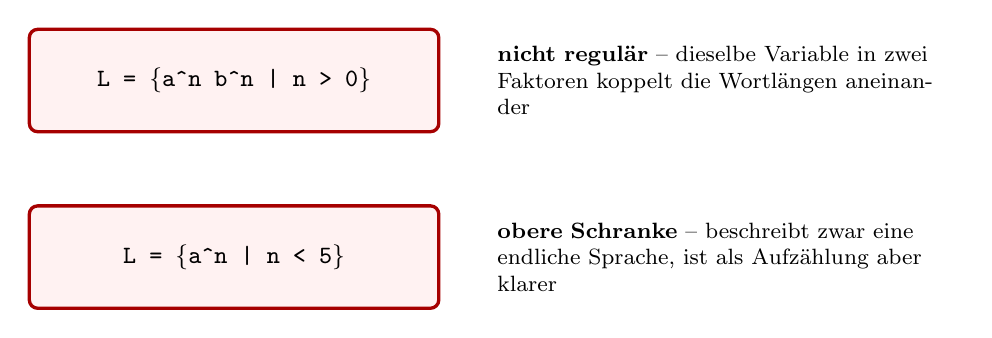
\begin{tikzpicture}[
        bad/.style={draw=red!65!black, very thick, rounded corners=3pt, fill=red!5,
                    minimum width=52mm, minimum height=13mm, font=\small\ttfamily},
        why/.style={font=\footnotesize, align=left, text width=58mm}
      ]
      \node[bad]                     (a) {L = \{a\^{}n b\^{}n | n > 0\}};
      \node[why, right=6mm of a]     (aw) {\textbf{nicht regulär} -- dieselbe Variable in zwei
                                            Faktoren koppelt die Wortlängen aneinander};

      \node[bad, below=9mm of a]     (b) {L = \{a\^{}n | n < 5\}};
      \node[why, right=6mm of b]     (bw) {\textbf{obere Schranke} -- beschreibt zwar eine endliche
                                            Sprache, ist als Aufzählung aber klarer};
    \end{tikzpicture}
  \end{center}

  \vspace{1mm}
  \footnotesize
  Beide Eingaben ließen sich formal verarbeiten. Sie werden trotzdem mit einer
  \textbf{eigenen Meldung} zurückgewiesen: Diese Fälle ausdrücklich zu erklären ist lehrreicher,
  als sie stillschweigend zu verwerfen.

              \note{
                \textbf{Person: }

                \textbf{Zeit:  min}

                \begin{itemize}
                  \item Hier ist die didaktische Begründung der Punkt, nicht die Technik.
                  \item a\^{}n b\^{}n ist das Standardbeispiel für eine nicht-reguläre Sprache -- gut geeignet, um zu zeigen,
                  \item dass das Werkzeug die Theorie ernst nimmt.
                  \item Mögliche Rückfrage: "Warum keine oberen Schranken?" -- Antwort: endlich, also regulär, aber die
                  \item Aufzählung ist die klarere Schreibweise; die Eingabesprache bleibt kleiner.
                \end{itemize}
              }
\end{fullframe}


% ---------------------------------------------------------------------------
% Fachmodul Zahlensysteme (Enrico Ebert)
%
% Inhaltlich abgeleitet aus Abschnitt 4.4 der Dokumentation
% (includes/04_Designentscheidungen/04_04.tex).
%
% Die Kurznotizen stehen in \note{...}. Sie sind standardmäßig unsichtbar.
% Zum Anzeigen in presentation.tex vor \begin{document} ergänzen:
%     \setbeameroption{show notes}
% oder für einen zweiten Bildschirm:
%     \setbeameroption{show notes on second screen=right}
% ---------------------------------------------------------------------------

\addsectionframe{Fachmodul: Zahlensysteme}

% ---------------------------------------------------------------------------
\begin{itemframe}{Zahlensysteme konfigurieren}
  \item Fünf Modi: \textit{Integers}, \textit{Negative}, \textit{Fractional}, \textit{IEEE-754} und \textit{Arithmetik}
  \item Eingaben je nach Basis mit Regex-Filtern validiert, Bitlänge explizit begrenzt
  \item Negative Zahlen in fester 8-Bit-Breite (Wertebereich $-128$ bis $127$, abgestimmt auf die Vorlesung)
  \item Berechnungen durchgängig mit \texttt{BigInt} statt \texttt{Number}: keine Rundungsfehler bei großen Zahlen
\note{
  \textbf{Person: Enrico}

  \textbf{Zeit: 1,5 min}

  \begin{itemize}
    \item Deckt Vorlesungsstoff ab: Basisumrechnung bis IEEE\,754
    \item 5 Modi: Integers, Negative, Fractional, IEEE-754, Arithmetik
    \item Eingaben basisgerecht validiert, Bitlänge begrenzt
    \item Negative: 8 Bit, Wertebereich -128 bis 127 (Vorlesung)
    \item Berechnungen mit \texttt{BigInt} statt \texttt{Number} -- keine Rundungsfehler
    \item Überleitung: Ablauf in der App zeigen
  \end{itemize}
}
\end{itemframe}

% ---------------------------------------------------------------------------
\begin{contentsframe}{Schrittausführung}
\centering
\vspace{3mm}
\resizebox{0.95\textwidth}{!}{%
\begin{tikzpicture}[node distance=15mm and 11mm]
  \node[diagramnode, minimum width=3.4cm, font=\normalsize] (select) {Modus + Eingabe\\wählen};
  \node[diagramnode, right=of select, minimum width=3.4cm, font=\normalsize] (validate) {Eingabe\\validieren};
  \node[diagramnode, right=of validate, minimum width=4.2cm, font=\normalsize] (steps) {Schritt-Objekte\\mit \texttt{BigInt}\\erzeugen};
  \node[diagramnode, right=of steps, minimum width=3.4cm, font=\normalsize] (render) {Rechengitter\\anzeigen};
  \node[diagramnode, below=20mm of validate, minimum width=3.4cm, font=\normalsize] (error) {Fehlermeldung\\mit Hinweis};
  \node[diagramnode, below=20mm of render, minimum width=3.4cm, font=\normalsize] (overflow) {Overflow-\\Warnbanner};

  \draw[diagramarrow] (select) -- (validate);
  \draw[diagramarrow] (validate) -- node[above, font=\small, text=black] {gültig} (steps);
  \draw[diagramarrow] (steps) -- (render);
  \draw[diagramarrow] (validate) -- node[left, font=\small, text=black] {ungültig} (error);
  \draw[diagramarrow] (render) -- (overflow);
  \draw[diagramarrow] (error.west) -| node[pos=0.25, below, font=\small, text=black] {korrigiert} (select.south);
\end{tikzpicture}%
}
\note{
 \textbf{Person: Enrico}

 \textbf{Zeit: 1 min}

 \begin{itemize}
   \item Ablauf in der App, nicht das Rechenverfahren
   \item Modus + Eingabe $\rightarrow$ validieren $\rightarrow$ Schritt-Objekte $\rightarrow$ Rechengitter
   \item Ungültige Eingabe = Hinweis, Nutzer korrigiert
   \item Stufen aufklappbar, i18n-Texte bleiben beim Sprachwechsel erhalten
   \item Overflow-Banner warnt, korrigiert nicht -- didaktisch bewusst
   \item Darstellung passt sich Modus an:
     \begin{itemize}
       \item Wandler: klassische Mathematik-Blöcke
       \item Arithmetik: farbcodiertes Rechengitter
       \item Negative: Vorzeichen, Einer-, Zweierkomplement
       \item IEEE-754: Sign / Exponent / Mantisse getrennt
     \end{itemize}
 \end{itemize}
}
\end{contentsframe}


\addsectionframe{Fachmodul: Kodierung}

% ---------------------------------------------------------------------------
\begin{itemframe}{Kodierung -- Überblick}
  \item Meine Erklärung
\end{itemframe}

% ---------------------------------------------------------------------------
% Fachmodul Disjunktive Normalform (Duy Tan Pham)
%
% Inhaltlich abgeleitet aus Abschnitt 4.6 der Dokumentation
% (includes/04_Designentscheidungen/04_06.tex).
% ---------------------------------------------------------------------------

\addsectionframe{Fachmodul: Disjunktive Normalform}

% ---------------------------------------------------------------------------
\begin{itemframe}{Disjunktive Normalform -- Überblick}
  \item Zwei Aufgabenmodi: Ausdruck $\rightarrow$ Wahrheitstabelle und Wahrheitstabelle $\rightarrow$ DNF
  \item Drei Ergebnisstufen: kanonische DNF, minimale DNF und optional global kleinste UND/ODER-Formel
  \item Minimierung mit Quine-McCluskey und Branch-and-Bound
  \item Semantische Prüfung erkennt logische Äquivalenz
  \item Begrenzung auf maximal 4 Variablen für exakte Synthese
  \note{
    \textbf{Person: Tan}

    \textbf{Zeit:  1 min}

    \begin{itemize}
      \item \textbf{Aufbau:} UND-Terme werden durch ODER verbunden
      \item \textbf{Zwei Wege:} Ausdruck zur Wahrheitstabelle oder Wahrheitstabelle zur DNF
      \item \textbf{Kanonisch:} Jede 1-Zeile ergibt einen vollständigen Term mit allen Variablen
      \item \textbf{Minimal:} Weniger Literale, exakt mit QMC + B\&B
      \item \textbf{Global:} Ausklammern erlaubt, daher nicht zwingend DNF
      \item \textbf{Äquivalenz:} Funktion über Wahrheitstabelle vergleichen
      \item \textbf{Grenze:} Bis vier Variablen garantiert optimal
    \end{itemize}
  }
\end{itemframe}

% ---------------------------------------------------------------------------
\begin{contentsframe}{Schrittausführung}
\centering
\vspace{1mm}
\resizebox{0.95\textwidth}{!}{%
\begin{tikzpicture}[node distance=15mm and 11mm]
  \node[diagramnode, minimum width=3.3cm, font=\normalsize] (input) {Ausgangsdaten:\\Formel oder Tabelle};
  \node[diagramnode, right=of input, minimum width=3.3cm, font=\normalsize] (ast) {Syntaxprüfung\\Parser \& AST};
  \node[diagramnode, right=of ast, minimum width=3.5cm, font=\normalsize] (table) {Referenztabelle\\1-Zeilen bestimmen};
  \node[diagramnode, right=16mm of table, minimum width=3.5cm, font=\normalsize] (cdnf) {Kanonische DNF\\(Vollminterme)};

  \node[diagramnode, below=15mm of input, minimum width=3.3cm, font=\normalsize] (student) {Antwort\\je nach Modus};
  \node[diagramnode, below=15mm of ast, minimum width=3.3cm, font=\normalsize] (check) {Prüfung: Werte, Form\\und Äquivalenz};
  \node[diagramnode, below=15mm of table, minimum width=3.8cm, font=\normalsize] (exact) {Global kleinste Form\\exakt bis 4 Variablen};
  \node[diagramnode, below=15mm of cdnf, minimum width=3.5cm, font=\normalsize] (qmc) {Minimale DNF\\QMC + B\&B};

  \draw[diagramarrow] (input) -- node[above, font=\small, text=black] {Formel} (ast);
  \draw[diagramarrow] (ast) -- (table);
  \draw[diagramarrow] (input.north) to[out=70, in=110]
    node[above, font=\small, text=black] {Tabelle} (table.north);
  \draw[diagramarrow] (table) -- node[above, font=\small, text=black] {1-Zeilen} (cdnf);
  \draw[diagramarrow] (cdnf) -- (qmc);
  \draw[diagramarrow] (table) --
    node[pos=0.52, right, xshift=2mm, font=\small, text=black] {Funktion} (exact);
  \draw[diagramarrow, dashed] (qmc) -- node[above, font=\small, text=black] {Obergrenze} (exact);

  \draw[diagramarrow] (student) -- (check);
  \draw[diagramarrow] (table) --
    node[pos=0.68, above, xshift=-2mm, font=\small, text=black] {Referenz} (check);
  \draw[diagramarrow] (check.south) to[out=215, in=325] node[below, font=\small, text=black] {Feedback \& Äquivalenz} (student.south);
\end{tikzpicture}%
}
\note{
  \textbf{Person: Tan}

  \textbf{Zeit:  1,5 min}

  \begin{itemize}
    \item \textbf{Ausdrucksmodus:} Referenztabelle erzeugen und eingegebene Werte vergleichen
    \item \textbf{Tabellenmodus:} Vorgegebene Tabelle direkt als Referenz verwenden
    \item \textbf{Gemeinsamer Weg:} 1-Zeilen werden zur kanonischen DNF
    \item \textbf{Minimal:} Primimplikanten bilden und exakt auswählen
    \item \textbf{Global:} Minimale DNF als Obergrenze, kleinere Formel exakt suchen
    \item \textbf{Feedback:} Form und logische Äquivalenz mit der Referenztabelle prüfen
  \end{itemize}
}
\end{contentsframe}

\addsectionframe{Fachmodul: Moore Mealy}

% ---------------------------------------------------------------------------
\begin{itemframe}{Moore Mealy -- Überblick}
  \item Meine Erklärung
\end{itemframe}

\addsectionframe{Fachmodul: Java}

% ---------------------------------------------------------------------------
\begin{itemframe}{Java -- Überblick}
  \item Meine Erklärung
\end{itemframe}


\addsectionframe{6. Interaktive Live-Demo}

\begin{itemframe}{Demo-Ziel: den Lernweg sichtbar machen}
  \item Eingabe verändern
    \vspace{1em}
  \item Schrittweise ausführen
    \vspace{1em}
  \item Zwischenschritte erklären
    \note{
      \textbf{Person: }

      \textbf{Zeit: 5min}

      \begin{itemize}
        \item test
        \item test
        \item test
      \end{itemize}
    }
\end{itemframe}

\addsectionframe{7. Ausblick}

\begin{itemframe}{Perspektiven und offene Punkte}
  \item Weitere Lernbereiche und Topics
    \vspace{1em}
  \item Mobile Nutzung verbessern
    \vspace{1em}
  \item Java Zeilensperrung implementieren
    \vspace{1em}
  \item Gamification
    \vspace{1em}
  \item Lernstandsverfolgung
    \vspace{1em}
  \item LMS-Anbindung
    \note{
      \textbf{Person: }

      \textbf{Zeit: 2 min}

      \begin{itemize}
        \item test
        \item test
        \item test
      \end{itemize}
    }
\end{itemframe}

\end{document}
